\documentclass[a4paper,11.5pt]{article}
\usepackage[latin1]{inputenc}
\usepackage[T1]{fontenc}
\usepackage[english]{babel}
\usepackage{graphicx}
\usepackage{amsmath}
\usepackage{amsfonts}
\usepackage{multirow}
\usepackage{booktabs}
\usepackage{bbold}
\usepackage{mathtools}
\usepackage{mathrsfs}
\usepackage{enumitem}
\usepackage{array}
\usepackage{float}

\setlength{\parindent}{0pt}
\DeclarePairedDelimiter{\floor}{\lfloor}{\rfloor}
\DeclarePairedDelimiter{\ceil}{\lceil}{\rceil}

\newcommand{\vt}{\boldsymbol}

\title{Digital Communications - HW4}
\author{Jacopo Pegoraro, Edoardo Vanin}
\date{04/06/2018}

\begin{document}

\maketitle




\begin{figure}[H]
	\begin{center}   
		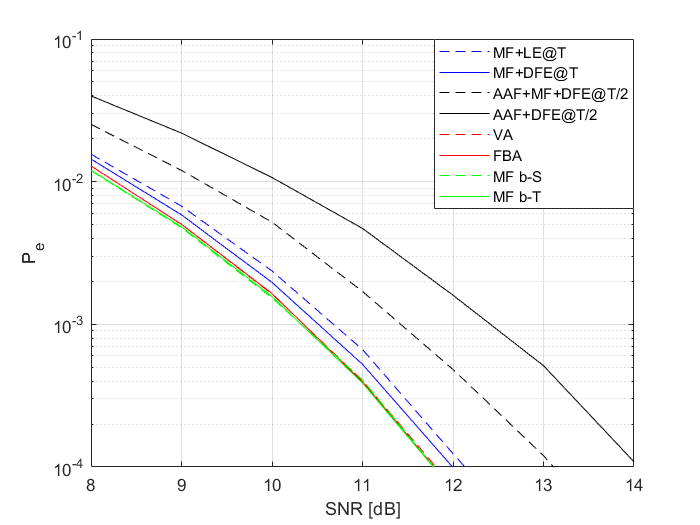
\includegraphics[width=\textwidth]{figs/SNR_Pe.png} 
		\caption{Results of the simulation over values of the SNR at the channel output from 8 dB to 14 dB.}
		\label{fig:SNR}
	\end{center}
\end{figure}


 
\begin{thebibliography}{15}
	
	\bibitem{nevio<3}
	Nevio Benvenuto, Giovanni Cherubini,
	\textit{Algorithms for Communication Systems and their Applications}. 
	Wiley, 2002.
	

	
\end{thebibliography}

\end{document}